\chapter{Fast graph kernel classifier based on optical random features }
\label{chapter:fast_algorithm}
\newtheorem{lemma}{Lemma} 
Graphlet kernel  is a good method to solve graph classification problem but as we have seen in chapter \ref{chapter:background}, it suffers from a high computational cost. In this chapter, we take inspiration from graph sampling and averaging to propose a family of fast graph kernels that generalizes the graphlet kernel paradigm. We show how random features can be incorporated within the new framework to get a faster and competitive algorithm in graph classification. Finally, we describe how Optical Processing Units (OPUs) can be used to eliminate some significant computational cost altogether.

\section{Proposed algorithm}
We recall from chapter \ref{chapter:background} that the computational cost of graphlet kernel is $C_{gk}= O(\tbinom{v}{k} N_k C_k)$. As an attempt to lower this cost, using graph sampling we can compute an empirical approximation of $k$-spectrum vector so the new that cost becomes $C_{gk + gs}= O(C_S s N_k C_k)$. We can see that $\tbinom{v}{k}$ is replaced with $C_S s$, and recall that the minimum number of samples $s \sim N_k$ required to ensure some certainty sharply increases as the graphlet size increase. It is clear then that the number of graph samples is not the only bottleneck here but also the cost to compute $\varphi_k^{match}$, denoted by $C_{\varphi_k^{match}}=O(N_k C_k)$.

So we propose to replace $\varphi^{match}_k$ with another user-defined function $\varphi:\phlet \mapsto\R^m$ and keep everything else as it is. We obtain a family of algorithms referred to as Graph Sampling and Averaging (GSA-$\varphi$), described in Alg. \ref{alg:GSA}, whose main user-defined methods are the samping method $S_k$ and the feature map $\varphi$.

\begin{algorithm}[H]\label{alg:GSA}
\DontPrintSemicolon
  \KwInput{2-Classes labelled graph dataset $\mathcal{X}=(\G_i,y_i)_{i=1,\ldots,n}$}
  \KwOutput{Trained model to classify graphs}
  \tools{Graph random sampler $S_k$, a function $\varphi$, linear classifier (ex. SVM) }\\
  \Hyp{k:graphlet size, $s$:\#graphlet samples per graph}\\
  %\KwData{Testing set $x$}
  %$\sum_{i=1}^{\infty} := 0$ \tcp*{this is a comment}
  %\tcc{}
  \Algo{\\}
  Random initialization of SVM weights\\
  \For{$\G_i$ in $\mathcal{X}$}{
  $\varphi_i=0$\\
  \For{$j=1:s$}{
  $F_{i,j}\gets S_k(\G_i)$\\
  $\varphi_i\gets \varphi_i +\frac{1}{s}\varphi(F_{i,j})$
  }
  }
  $\mathcal{D}_{\varphi}\gets (\varphi_i,Y_i)_{i=1,\ldots, n}$\\
  Train the linear classifier on the new vector-valued dataset $\mathcal{D}_{\varphi}$
\caption{Graph Sampling and Averaging (GSA-$\varphi$)}
\end{algorithm}

For a set $\mathfrak{F} = \{F_1,\ldots, F_s\}$ and a feature map $\varphi$, similarly to $\bm{\varphi}^{hist}$ we define $\bm{\varphi}(\mathfrak{F}) = \frac{1}{s} \sum_i \varphi(F_i)$. The GSA-$\varphi$ algorithm computes, for each graph $\G$ in the dataset, an embedding $\bm{\varphi}(\mathfrak{F}_\G)$ where $\mathfrak{F}_\G$ is a set of $s$ subgraphs drawn $iid$ from $S_k(\G)$, then trains a classifier on it.

We note that within the new paradigm, the defined $\varphi$ does not necessarily respect the isomorphism between sampled subgraphs: if $\varphi(F) = \varphi(F')$ whenever $F \cong F'$, then we are in the framework of graphlet \emph{without} repetition, otherwise we are in the other case. As we will see, choosing a randomized $\varphi$ presents both theoretical and practical advantages, however it does not respect isomorphism. Nevertheless, it is possible to apply some preprocessing function $Q$ invariant by permutation before passing it to a randomized $\varphi$, and in this case isomorphism is respected without any condition on $\varphi$. An example of such function is $Q:\R^{k\times k}\mapsto \R^k, Q(F)=Sort(Eigenvalues(\mathbf{A}_F))$, that is, the sorted eigenvalues of the adjacency matrix.

\todoNK{A word on the generic computational cost of the method ? $O(C_S s C_\varphi)$, emphasizing that $C_\varphi$ is now the main focus in the rest (intuitively, trade off between computational cost and discriminative power)}

\section{Using random features framework in our algorithm}

In the previous section, we introduced a generic family of algorithms, GSA-$\varphi$. Besides the sampling method, the performance and computational cost of the algorithm mainly depends on the choice of feature map $\varphi$: choosing $\varphi = \varphi^{match}_k$ produces the classical graphlet kernel but it is expensive to compute. In this section, we motivate the choice of $\varphi$ as kernel random features  and relate it to a new notion of metric between graphs, using the so-called \emph{Maximum Mean Discrepancy} (MMD) \citep{gretton}, a kernel metric between probability distributions.

Let us recall a few notions about kernel RF (see Section \ref{sec:RF}). Assume that we have a psd (often shift-invariant) kernel on $\R^{k \times k}$, that can be written in the form:
\begin{equation}
\label{eq:random_features_3}
\mathcal{K}(F,F')= \mathbb{E}_{w \sim p(w)} \xi_w(F)^* \xi_w(F')
\end{equation}
for some mapping $\xi_w : \R^{k \times k} \to \mathbb{C}$ parameterized by $w$ distributed according to $p(w)$. Although this kernel technically takes (the adjacency matrix of) a graphlet as an input, we do not require it to be permutation-invariant, since it will be combined with the graph sampling process. For instance, we will see in experiments that even a simple Gaussian kernel on adjacency matrices performs well!

As we have seen, the RF method defines:
\begin{equation}\label{eq:RF}
\varphi(F) = \frac{1}{\sqrt{m}} ( \xi_{w_j}(F) )_{j=1}^m \in \mathbb{C}^m,~~~ m\in \mathbb{N}
\end{equation}
and we can write:
\[
\mathcal{K}(F,F')\approx \varphi(F)^*\varphi(F')
\]

Now, how does the embedding computed by GSA-$\varphi$ relates to the base kernel $\mathcal{K}$? To examine that, in the following we define another kernel, called the \emph{mean kernel} $\K_{mk}$ \citep{gretton}, with its corresponding metric called the \emph{Maximum Mean Discrepancy (MMD)}. Next, we show with the aid of concentration inequalities how using the random features map $\varphi$ of $\K$ in our algorithm GSA-$\varphi$ will lead to an approximation of $\K_{mk}$ concentrated around its true value with high probability.

The mean kernel methodology allows to \emph{lift} a kernel from a domain $\phlet$ to a kernel on \emph{probability distributions} on $\phlet$. Given a base kernel $\K$ on $\phlet$ and two probability distribution $\mathcal{P},\mathcal{Q}$, it is defined as:
\begin{equation}
\label{eq:mean_kernel}
\mathcal{K}_{mk}(\mathcal{P},\mathcal{Q}) = \mathbb{E}_{x \sim \mathcal{P}, y \sim \mathcal{Q}} \mathcal{K}(x,y)
\end{equation}
In other words, the mean kernel is just the expectation of the base kernel with respect to each term. The metric associated to the mean kernel is usually referred to as the \emph{Maximum Mean Discrepancy (MMD)} in the literature \citep{gretton}, and is defined as:
\begin{equation}\label{eq:MMD}
MMD(\mathcal{P},\mathcal{Q}) = \sqrt{\mathcal{K}_{mk}(\mathcal{P},\mathcal{P}) + \mathcal{K}_{mk}(\mathcal{Q},\mathcal{Q}) - 2\mathcal{K}_{mk}(\mathcal{P},\mathcal{Q})}
\end{equation}
It should be noticed here that $\mathcal{K}_{mk}(\mathcal{P},\mathcal{P}) = \mathbb{E}_{x \sim \mathcal{P}, x' \sim \mathcal{P}} \mathcal{K}(x,x') \neq \mathbb{E}_{x \sim \mathcal{P}} \mathcal{K}(x,x)$.

\textbf{The link between the mean kernel and graph sampling} can be easily constructed, since considering a random sampling method $S_k$, the pair $(S_k , \G)$  introduces a probability distribution $f_\G= \mathbb{E}_{F \sim S_k(\G)} \varphi^{match}_k(F)$ on the set of size-$k$ graphlets $\phlet$. Thus, for two graphs $\G,\G'$ , the mean kernel between these distributions, denoted by $\mathcal{K}_{mk}(\G,\G')=\mathcal{K}_{mk}(f_\G,f_{\G'})$ for simplicity, can be reformulated as:
\begin{equation}
\label{eq:mean_kernel_graphs}
\mathcal{K}_{mk}(\G,\G') = \mathbb{E}_{F \sim S_k(\G), F' \sim S_k(\G')} \mathcal{K}(F,F')
\end{equation}
Remark that the mean kernel also reduces to:
\[
\mathcal{K}_{mk}(\G,\G')=\sum_{i,j}^{N_k}(f_\G)_i(f_{\G'})_j\mathcal{K}(\phlet_i,\phlet_j) 
\]
We denote by $MMD(\G,\G')$ the corresponding MMD, which is a new notion of distance between graphs that generalizes the graphlet kernel metric.

Let us now integrate random features with the mean kernel, assuming \eqref{eq:random_features_3} and \eqref{eq:RF}, and show how GSA-$\varphi$ relates to the MMD we have just defined. We combine the decomposition of the base kernel $\mathcal{K}$ in Eq. \eqref{eq:random_features_3} with Eq. \eqref{eq:mean_kernel_graphs} to get:
\begin{equation}
    \label{eq:mk_rf}
    \mathcal{K}_{mk}(\G,\G')= \mathbb{E}_{F \sim S_k(\G), F' \sim S_k(\G')} \mathbb{E}_w \xi_w(F)\xi_w(F')
\end{equation}
The corresponding MMD metric in this case is:
\begin{equation}
\label{eq:MMD-RF}
MMD(\G,\G')^2 = \mathbb{E}_{\omega} \Big( | \mathbb{E}_{S_k(\G)} \xi_\omega(F) - \mathbb{E}_{S_k(\G')} \
\xi_\omega(F') |^2 \Big)
\end{equation}

Until now, what we have in Eq. \ref{eq:mk_rf} is the true value of the mean kernel, where the expectations there implies that we should consider infinite number of both graph samples and random features. However, what we really want is to approximate this value using our algorithm GSA-$\varphi$, which includes  using the finite-dimensional map $\varphi$ and a finite number of \emph{iid} samples drawn with $S_k$. First let's consider only a finite number $s$ of samples: $\F_\G=\{F_1, \ldots, F_s\}$ and $\F_{\G'}=\{F'_1, \ldots, F'_s\}$. Then we have: 
\begin{equation}
\label{eq:MK_samples}
\mathcal{K}_{mk}(\G,\G') \approx \frac{1}{s^2} \sum_{i,j=1}^s \mathbb{E}_w \xi_w(F_i)\xi_w(F'_j)
\end{equation}
\[
MMD(\G,\G')^2 \approx \frac{1}{s^2}\mathbb{E}_{\omega} ( | \xi_\omega(F) -\xi_\omega(F') |^2 )
\]
No we consider both a finite number $s$ of \emph(iid) samples, and a feature map $\varphi$ with finite number $m$ of random features defined as \eqref{eq:RF}, so the formula of our final approximation is:
\begin{equation}
\label{eq:mean_kernel_RF}
\mathcal{K}_{mk}(\G,\G') \approx \frac{1}{s^2} \sum_{i,j=1}^s \varphi(F_i)^*\varphi(F_j')=\Big(\frac{1}{s}\sum_{i=1}^s\varphi(F_i)\Big)^*~\Big(\frac{1}{s}\sum_{i=1}^s\varphi(F_i')\Big) = \bm{\varphi}(\mathfrak{F}_{\G})^* \bm{\varphi}(\mathfrak{F}_{\G'})
\end{equation}
\[
MMD(\G,\G')^2 \approx  \| \bm{\varphi}(\mathfrak{F}_{\G}) - \bm{\varphi}(\mathfrak{F}_{\G'}) \|_2^2 
\]
Indeed, we just proved that, when using random features, GSA-$\varphi$ theoretically represents an unbiased estimation of the mean kernel $\mathcal{K}_{mk}$. The corresponding MMD is then the key to the performance of the algorithm: if the graphs are well-separated by this metric, then a machine learning algorithm will be able to classify them.

Now, we have two issues to discuss: how is this estimation concentrates around its expected value $\mathcal{K}_{mk}$, and what is the computational cost of GSA-$\varphi$ in this case. While the first question can be addressed for any kernel $\mathcal{K}$, the second one is really case-dependent as it is mainly related to the computational cost of computing the term $\varphi(F_i)$ in Eq. \eqref{eq:mean_kernel_RF} which differs from one $\varphi$ to another \todoNK{I would define the generic cost $C_\varphi$ in the previous section and keep the discussion focused on concrete examples of RF here (Gaussian, gaussian with eigenvalues...)}. We start answering the first question.

\begin{theorem}
\label{theorem:concentration}
Let $\G$ and $\G'$ be two graphs, $\{F_i\}_{i=1}^{s}$ (resp. $\{F_i'\}_{i=1}^{s}$) be $iid$ size-k graphlet samples drawn from $S_k(\G)$ (resp. $S_k(\G')$). Assume a kernel of the form \eqref{eq:random_features_3} and a random feature map \eqref{eq:RF}. Assume that $\abs{\xi_w(F)} \leq 1$ for any $w,F$.

We have that, for all $\delta>0$, with probability at least $1-\delta$:
\begin{align*}
 \Big|\|\varphi(\mathfrak{F}_\G) - \varphi(\mathfrak{F}_{\G'})\|^2 - MMD(\G,\G')^2 \Big| \leq \frac{4 \sqrt{\log (6/\delta)}}{\sqrt{m}} + \frac{8\left(1+\sqrt{2\log(3/\delta)}\right)}{\sqrt{{s}}}
\end{align*}
\end{theorem}
this tells that the Euclidean distance between embedding computed by GSA-$\varphi$ converges to the MMD in $O(1/\sqrt{m} + 1/\sqrt{s})$. The proof of this theorem is provided in section \ref{section:proof}.

<<<<<<< HEAD
To calculate \textbf{the computational cost of $GSA-\varphi$}, we considered three cases of $\varphi$ in our experiments, hence $\mathcal{K}$, in both theoretical and practical sides: Gaussian random features applied on the adjacency matrix, Gaussian random features applied on the sorted Eigenvalues of the adjacency matrix , and finally the optical random features of OPUs. The case of OPU random features is presented in section \ref{section:OPU}.\newline
\todome{
here am supposed after few words to reach the point:
$C_{\varphi_{Gs}}=O(mk^2)$ for the adjacency matrix
and 
$C_{\varphi_{Gs}}=O(mk^2+C_{Eigen_extraction})$ for the adjacency matrix}
\todoNK{you can use the theorem above to say that $m$ should be of the order of $s$ (since the error rate is the same in $m$ and $s$), which is high. Hence the huge gain with the OPU.}
=======
To calculate \textbf{the computational cost of $GSA-\varphi$}, we considered three cases of $\varphi$, hence $\mathcal{K}$, in both theoretical and practical sides: Gaussian random features applied on the adjacency matrix, Gaussian random features applied on the Eigenvalues of the adjacency matrix , and finally the optical random features of OPUs. The case of OPU random features is presented in section \ref{section:OPU}.\newline
For a flattened version of an adjacency matrix $\mathbf{A}_{flat}$ of a subgraph $F$, we recall that the Gaussian kernel stated in Eq. \ref{eq:Guassian_kernel} can be approximated by the inner product of the following random features map:
\[
\varphi(\mathbf{A}_{flat}) = \frac{1}{\sqrt{m}} ( \sqrt{2}cos(w_j^T\mathbf{A}_{flat}+b) )_{j=1}^m \in \mathbb{C}^m
\]
where $w_j\in\R^{k^2}$ drawn from the Gaussian distribution in Eq. \ref{eq:G_fourier}. Hence, The computational cost needed in this case for each subgraph to compute its $\varphi(\mathbf{A}_{flat})$ is $O(mk^2)$ . Which is the cost of matrix multiplication supposing that we have a fast method to evaluate the $cos$ function. Finally, the processing cost per graph $\G$ is: $C_{Gs}=O(smk^2)$.

Gaussian random features applied on the Eigenvalues of the adjacency matrix is similar to the one applied on the adjacency matrix, the difference is that instead of passing the adjacency matrix as an input, we pass a vector of its Eigenvalue $\boldsymbol{\lambda}\in\R^k$. So what changes per subgraph process is the input dimension and the cost of Eigenvalues extraction, which is $O(k^3)$. In a similar way, we can write: $C_{Gs+Eig}=O(s(mk+k^3))$.

>>>>>>> 212a4937ba12b07559998ab673b99f81e8f360f4


\section{Fast $GSA-\varphi$ with optical random features}
\label{section:OPU}
Optical processing units (OPUs) are physical units developed to apply optical random features projections in light-speed. In this section and before introducing $GSA-\varphi$ in its ultimate and fastest form $GSA-\varphi_{OPU}$, we explain what optical random features projection is. We start by presenting the mathematical model of these projections $\varphi_{OPU}$, next we explain how OPUs can perform such projections in light-speed from hardware point of view. Finally, we merge OPUs' random features with our proposed algorithm and compare the corresponding computational cost with previously mentioned methods.

\subsection{Optical random features model}
Random projections is one of the important techniques in machine learning and in signal processing. However, traditional random projection methods need a large memory to store the corresponding random matrix $\mathbf{W}$ and a huge computational time to project the input data points $\mathbf{x}$, i.e. to compute $\mathbf{Wx}$. Optical processing units (OPU's) is the technology developed to solve the previous two drawbacks: where an OPU complete random projections at the speed of light without the need to store any random matrix. In general, Random projections are the result of two procedures: the first one is the linear-random projections and the second one is non-linear mapping.
Mathematically speaking, OPU's perform the following operation \citep{saade_opu}:
\begin{equation}
\label{OPU_equation}
\mathbf{\varphi}_{OPU}(\mathbf{x})=|\mathbf{Wx+b}|^2 ;~\mathbf{W}\in \mathbb{R}^{m\times d},\mathbf{b}\in \mathbb{R}^m, \mathbf{x}\in \mathbb{R}^d
\end{equation}
Where $\mathbf{b}$ is a bias vector, $\mathbf{x}$ is an input point, $m$ is the number of random features, $d$ is the input space dimension and the amplitude function $|.|$ is taken element wise in $\mathbf{\varphi}_{OPU}(\mathbf{x})$. The matrix $\mathbf{W}$ is a random \emph{iid} complex matrix with Gaussian real and imaginary parts.\newline
In the limit where the number of random features $m\xrightarrow{}\infty$, it can be proven by the concentration of the measure that the inner product between the projected data points $(\mathbf{\varphi}_{OPU}(\mathbf{x}\in \mathbb{R}^m)$ in the new feature space tends to a kernel function that depends only on the input points in the original feature space $(\mathbf{x}\in \mathbb{R}^d)$

\subsection{OPU structure and functionality}
Eq.~\ref{OPU_equation} still imply that an OPU need to store and multiply by the random projection matrix. But in an OPU, a heterogeneous material, as a paper or any white translucid material, is used to scatter incident light in a very complex way. The behavior of the scattering process is considered random because of the extremely high complexity. One can argue that light scattering is a linear, deterministic, and reproducible phenomenon, but what can be said here is that the unpredictable behavior of the process makes it effectively a random process. That is why these materials are called opaque since all information embedded within the incident light is seemingly lost during the propagation through the material \citep{saade_opu}. An example used to demonstrate and justify the resulted randomness is a cube of edge length $100\mu m$, such cube can include $\approx 10^7$ paint nanoparticles, all the positions and shape of these particles must be known in order to predict its effect on light. Propagation through such a layer can be seen as a random walk because of frequent scattering with the nanoparticles, where light explores the whole volume and undergoes tens of thousands of such scattering steps before coming out from the other side in a few picoseconds.\newline

\begin{figure}[ht!]
\begin{center}
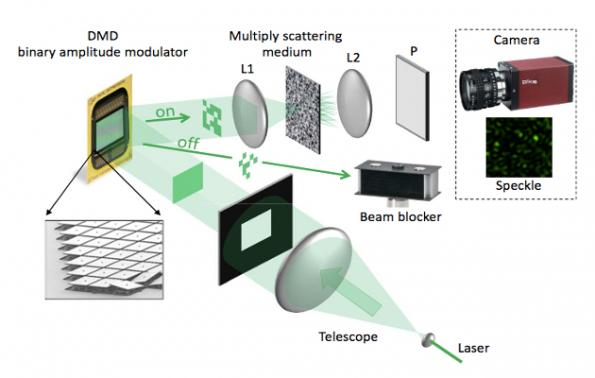
\includegraphics[scale=0.5]{figs/lighton630.jpg}
\end{center}
\caption[OPU's Experimental setup]{OPU's Experimental setup \citep{saade_opu}: A monochromatic laser is expanded by a telescope, then
illuminates a digital micromirror device (DMD), able to spatially encode digital information on the light beam by
amplitude modulation. The light beam carrying the signal is then focused on a random
medium by means of a lens. The transmitted light is collected on the
far side by a second lens, passes through a polarizer, and is measured by a standard monochrome CCD camera for example .}
\label{fig_opu}
\end{figure}
When the incident light is coherent, it promotes complex interference patterns, called speckles, due to the scattering process.
These speckles don't only characterize the propagation medium but also the incident light, and this can be modeled by $y=Wx$, 
where $y$ and $x$ are the vector amplitudes between a set of spatial modes at the output and at the input of the medium respectively. In OPUs, the transmission matrix $W$ of the propagation medium can be approximately considered as a Gaussian i.i.d matrix, it was also shown that even without $W$ being known, but it is guaranteed to be stable as long as the propagation medium is stable as a paint layer for instance \citep{saade_opu}.  So if we use a spatial light modulator and a laser to send an appropriate set of illuminations to the propagation medium, we can acquire the output intensity $|y|^2$ with a CCD or CMOS camera, and that is the principle concept behind OPU's functionality as seen in Fig~ \ref{fig_opu}.\newline 
The DMD (digital micromirror device) used in OPU's is a binary amplitude modulator consisting of an array of micro-mirrors, Each mirror can be lit or not, thus it can represent  a binary value. In order to represent grey values, each value is encoded on a square sub-array ($4\times 4$ for example) in the DMD, where the number of lit mirrors reflects the desired level of grey. DMD reflects the data and send the reflected light through the disordered medium, then a snapshot of the resulting random projection is acquired using a standard camera. all that is completed in a very high speed compared to the traditional random features techniques. 
\subsection{Fast $GSA-\varphi_{OPU}$ algorithm with complexity discussion}
After what we presented about OPUs and optical random features projections, we can efficiently deploy $\varphi_{OPU}$ random feature map in $GSA-\varphi$ framework. The resulted pseudo code is presented below and we refer to the resulted algorithm with $GSA-\varphi_{OPU}$. \newline\newline
\begin{algorithm}[H]
\DontPrintSemicolon
  \KwInput{2-Classes labelled graph dataset $\mathcal{X}=(\G_i,y_i)_{i=1,\ldots,n}$}
  \KwOutput{Trained model to classify graphs}
  \tools{Graph random sampler $S_k$, optical processing unit (OPU), linear classifier (ex. SVM) }\\
  \Hyp{k:graphlet size, $s$:\#graphlet samples per graph}\\
  %\KwData{Testing set $x$}
  %$\sum_{i=1}^{\infty} := 0$ \tcp*{this is a comment}
  %\tcc{}
  \Algo{\\}
  Random initialization of the classifier weights\\
  \For{$\G_i$ in $\mathcal{X}$}{
  $\boldsymbol{\varphi}_{OPU}(i)=0$\\
  \For{$j=1:s$}{
  $F_{i,j}\gets S_k(\G_i)$\\
  $\mathbf{A}\gets adjacency\_matrix(F_{i,j})$\\
  $\boldsymbol{\varphi}_{OPU}(i)\gets \boldsymbol{\varphi}_{OPU}(i) +\frac{1}{s}\boldsymbol{\varphi}_{OPU}(F_{i,j})$
  }
  }
  $\mathcal{D}_{\varphi_{OPU}}\gets (\boldsymbol{\varphi}_{OPU}(i),y_i)_{i=1,\ldots, n}$\\
  Train the linear classifier on the new vector-valued dataset $\mathcal{D}_{\varphi_{OPU}}$
\caption{GSA-$\varphi_{OPU}$}
\end{algorithm}

\textbf{The computational cost} of this innovative version $GSA-\varphi_{OPU}$, and more specifically of computing $\boldsymbol{\varphi}_{OPU}(\mathbf{A})$, is $O(1)$ in both the number of random features and the graphlet size. One can reasonably argue that an OPU has its limits, as the DMD mirror array ,where the input $\mathbf{A}$ is encrypted, has a limited dimensions \emph(width $\times$ length). Moreover, the camera used to acquire the light intensity in an OPU has a limited number of pixels thus it introduces a limit on the maximum number of random features. However, our argument is that when we respect these limits, which are usually large ones, the computational cost is a constant in both $m$ and $k$. To better illustrate the advantage of $GSA-\varphi_{OPU}$ over other discussed methods in this work, we show a comparison between them with respect to the computational time per graph $\G$:
\begin{itemize}
    \item Graphlet kernel: $C_{gk}= O(\tbinom{v}{k} N_k C_k)$
    \item Graphlet kernel with sampling: $ C_{gk + gs}= O(C_s s N_k C_k)$
    \item Gaussian features $GSA_{\varphi_{Gs}}$: $C_{Gs}=O(smk^2)$
    \item Gaussian features  $GSA_{\varphi_{Gs}}$ with Eigenvalue preprocessing: $C_{Gs+Eig}=O(s(mk+k^3))$
    \item $GSA_{\varphi_{OPU}}$:  $C_{OPU}=O(1)$
\end{itemize}

\section{$GSA-\varphi$ concentration inequality proof}
\label{section:proof}

\begin{proof}
<<<<<<< HEAD
Here, we prove theorem \ref{theorem:concentration}. We decompose the proof in two steps.

\paragraph{Step 1: infinite $s$, finite $m$ (number of random features).} Based on our assumption $|\xi_w|\leq 1$, it is a straightforward result of Hoeffding's inequality that  $MMD(\G, \G')^2$ is close to $\frac{1}{m} \sum_{j=1} | \mathbb{E}_{F \sim S_k(\G)} \xi_{w_j}(F) - \mathbb{E}_{F' \sim S_k(\G')}} \xi_{w_j}(F') |^2 = | \mathbb{E}_{F \sim S_k(\G)} \xi_{w_j}(F) - \mathbb{E}_{F' \sim S_k(\G')}} \xi_{w_j}(F') |^2$. We recall Hoeffding's inequality below.
=======
Here, we prove theorem \ref{theorem:concentration}, where We decompose the proof in two steps.
we first assume that:
\begin{equation}
\label{eq:z_assumption}
    0\leq z_\omega(F)\leq 1, \forall \omega \sim  \Lambda
\end{equation}
This is a reasonable assumption from what we have seen in random Fourier features maps referred to in Eq. \ref{eq:Fourier_xi}.
\paragraph{Step 1: infinite $s$, finite $m$ (number of random features).} Based on our assumption on $z_\omega$ in \eqref{eq:z_assumption}, it is a straight forward result of Hoeffding's inequality that  $d(G, G')^2$ is close to $\frac{1}{m} \sum_{j=1} | \mathbb{E}_{F \sim f_G} z_{\omega_j}(F) - \mathbb{E}_{F' \sim f_{G'}} z_{\omega_j}(F') |^2 = \| \mathbb{E}_{F \sim f_G} z(F) - \mathbb{E}_{F' \sim f_{G'}} z(F')\|^2$.  
>>>>>>> 212a4937ba12b07559998ab673b99f81e8f360f4
\begin{lemma}[Hoeffding's inequality] 
Let $(x_1,\ldots, x_m)$ be independent random variables such that the variable $x_i$ is strictly bounded by the interval $[a_i , b_i]$, and let $\overline{X}=\frac{1}{m}\Sigma_{i=1}^{m}x_i$ then we have:
\begin{equation}
\label{eq:Hoeffding}
    \mathbb{P}(|\mathbb{E}\overline{X}-\overline{X}|\geq \epsilon)\leq 2~ \exp \left(-\frac{2m^2\epsilon^2}{\Sigma_{i=1}^m(b_i-a_i)^2)} \right)
\end{equation}
\end{lemma}
%\begin
In our case, we define the variables $x_j=| \mathbb{E}_{F \sim S_k(\G)} \xi_{w_j}(F) - \mathbb{E}_{F' \sim S_k(\G')}} \xi_{w_j}(F') |^2$. They are independent, have expectation $MMD(\G,\G')^2$, and are bounded by the interval $[0,4]$, thus we have:
\begin{equation*}
    \mathbb{P}\left(\Big|\frac{1}{m} \sum_{j=1}^m | \mathbb{E}_{F \sim S_k(\G)} \xi_{w_j}(F) - \mathbb{E}_{F' \sim S_k(\G')}} \xi_{w_j}(F') |^2 - MMD(\G,\G')^2 \Big| \geq \epsilon\right) \leq 2~ e^{ -2m\epsilon^2/16}
\end{equation*}
Or, in other words, with probability $1-\delta$,
\begin{equation}\label{eq:step1}
\Big|\frac{1}{m} \sum_{j=1}^m | \mathbb{E}_{F \sim S_k(\G)} \xi_{w_j}(F) - \mathbb{E}_{F' \sim S_k(\G')} \xi_{w_j}(F') |^2 - MMD(\G,\G')^2 \Big| \leq \frac{4 \sqrt{\log (2/\delta)}}{\sqrt{m}}
\end{equation}

\paragraph{Step 2: finite ${s}$ and $m$.} We show that for any \emph{fixed} set of random features $w_j$, we have $\| \mathbb{E}_{F \sim S_k(\G)} \varphi(F) - \mathbb{E}_{F' \sim S_k(\G')} \varphi(F')\|$ close to $\| \frac{1}{{s}} \sum_i \varphi(F_i) - \frac{1}{{s}} \sum_i \varphi(F'_i)\|$. 
%Let us consider a fixed set of random variables $\{\omega_j\}_{j \in \{1,\ldots, m\}}$ drawn independently from $\Lambda$, thus the random features map of a graph F equals: $z(F) = \frac{1}{\sqrt{m}}\left[z_{\omega_j}(F)\right]_{j=1}^m$.\newline
By definition of $F_1,\ldots, F_{s}$ random subgraphs drawn independently from $S_k(\G)$, we clearly have: 
\begin{equation}
\label{eq:subsample}
    \mathbb{E}_{F \sim S_k(\G)} \varphi(F)= \mathbb{E} (~\frac{1}{{s}} \sum_i \varphi(F_i)~)
\end{equation} 
Moreover by our assumptions $\varphi(F)$ is in a ball of radius $M=\frac{\sqrt{m}}{\sqrt{m}}=1$. We the apply the following vector version of Hoeffding's inequality.
\begin{lemma}
\label{lemma:vector_hoeffding}
let $X=\{x_1,\ldots,x_{s}\}$ be $iid$ random variables in a ball of radius $M$ centered around the origin in a Hilbert space $\mathcal{H}$. Denote their average by $\overline{X}=\frac{1}{{s}}\sum_{i=1}^{s}x_i$. Then for any $\delta>0$, with probability at lest $1-\delta$, 
\begin{equation}
\label{eq:vector_hoeffding0}
  \| \overline{X}-\mathbb{E}\overline{X}\|_\mathcal{H} \leq \frac{M}{\sqrt{{s}}}\left(1+\sqrt{2\log\frac{1}{\delta}}\right)
\end{equation}
\end{lemma}
\begin{proof}
Although this lemma is known in the literature, we reproduce its proof for completeness. Defining the function $f(x)= \| \overline{X}-\mathbb{E}\overline{X}\|$, and $\widetilde{X}={x_1,\ldots,\widetilde{x}_i,\ldots,x_{s}}$ to be a copy of $X$ with the ith element replaced by an arbitrary element of $\mathcal{H}$, we can prove using the triangle inequality:
\begin{equation}
    |f(X)-f(\widetilde{X})|=\Big|\| \overline{X}-\mathbb{E}\overline{X} \|-\|\overline{\widetilde{X}} - \mathbb{E}\overline{X}  \| \Big|\leq \| \overline{X} - \overline{\widetilde{X}}\|\leq
    \frac{\|x_i - \widetilde{x_i} \|}{{s}}\leq
    \frac{2M}{{s}}
\end{equation}
Therefore, $f(X)$ is insensitive to the ith component of $X,~ \forall i \in \{1,\ldots,{s}\}$ which suggests applying McDiarmid's inequality on $f$.

To bound the expectation of $f$, we use the familiar identity about the variance of the average of $iid$ random variables:
\begin{equation}
\mathbb{E}\|\overline{X}-\mathbb{E}\overline{X}\|^2=\frac{1}{n}(\mathbb{E}\|x\|^2-\|\mathbb{E}x\|^2 ) 
\end{equation}
Also:
\[ \mathbb{E}f(X)\leq\sqrt{\mathbb{E}f^2(X)}=\sqrt{\mathbb{E}\|\overline{X}-\mathbb{E}\overline{X}\|^2}\leq \frac{M}{\sqrt{{s}}}\]
This bound for the expectation of $f$ and McDiarmid's inequality give: 
\begin{equation}
\label{eq:vector_hoeffding1}
    \mathbb{P}_x \Big [ f(X)-\frac{M}{\sqrt{{s}}}\geq \epsilon \Big ]\leq
    \mathbb{P}_x \Big [ f(X)-\mathbb{E}f(X)\geq \epsilon \Big ]\leq
    \exp\Big( -\frac{{s}\epsilon^2}{2M^2}\Big)
\end{equation}
Which is equivalent to \eqref{eq:vector_hoeffding0} by setting $\delta=exp( -\frac{{s}\epsilon^2}{2M^2})$ and solving for $\epsilon$.
\end{proof}
Now back to Eq. \eqref{eq:subsample} and its corresponding assumptions that we made, we can directly apply lemma \ref{lemma:vector_hoeffding} (and more especially Eq.\eqref{eq:vector_hoeffding1}) to get that with probability $1-\delta$:
\begin{equation}
    \label{eq:fixed_w}
    \|\mathbb{E}_{F \sim S_k(\G)} \varphi(F)-~\frac{1}{s} \sum_i \varphi(F_i)~\|\geq \frac{1}{\sqrt{{s}}}\left(1+\sqrt{2\log\frac{1}{\delta}}\right)
\end{equation}
Now, by a union bound and triangle inequality: with probability $1-2\delta$,
\begin{align*}
    \Big | \| \mathbb{E}_{F \sim S_k(\G)} \varphi(F)& - \mathbb{E}_{F' \sim S_k(\G')} \varphi(F')\| - \| \frac{1}{{s}} \sum_i \varphi(F_i) - \frac{1}{{s}} \sum_i \varphi(F'_i)\|\Big | \\
    &\leq  \| \mathbb{E}_{F \sim S_k(\G)} \varphi(F) -  \frac{1}{{s}} \sum_i \varphi(F_i) \| + \|\mathbb{E}_{F' \sim S_k(\G')} \varphi(F') - \frac{1}{{s}} \sum_i \varphi(F'_i)\| \\
    &\leq \frac{2}{\sqrt{{s}}}\left(1+\sqrt{2\log\frac{1}{\delta}}\right)
\end{align*}
Moreover, since $\| \mathbb{E}_{F \sim S_k(\G)} \varphi(F)- \mathbb{E}_{F' \sim S_k(\G')} \varphi(F')\| + \| \frac{1}{{s}} \sum_i \varphi(F_i) - \frac{1}{{s}} \sum_i \varphi(F'_i)\| \leq 4$, with the same probability:
\begin{equation}\label{eq:step2}
    \Big | \| \mathbb{E}_{F \sim S_k(\G)} \varphi(F) - \mathbb{E}_{F' \sim S_k(\G')} \varphi(F')\|^2 - \| \frac{1}{{s}} \sum_i \varphi(F_i) - \frac{1}{{s}} \sum_i \varphi(F'_i)\|^2\Big | \leq \frac{8}{\sqrt{{s}}}\left(1+\sqrt{2\log\frac{1}{\delta}}\right)
\end{equation}
%Thus, since the two variables $\| \mathbb{E}_{F \sim f_G} z(F) -  \frac{1}{{s}} \sum_i z(F_i) \|$ and $\|\mathbb{E}_{F' \sim f_{G'}} z(F') - \frac{1}{{s}} \sum_i z(F'_i)\|$ are independent (as a direct result of our aforementioned assumption of independent random sampling), $\forall \epsilon>0$ we have:
%\begin{align*}
%    Pr( \| \mathbb{E}_{F \sim f_G} z(F) -  \frac{1}{{s}} \sum_i z(F_i) \| \geq \frac{1}{\sqrt{{s}}}+\frac{\epsilon}{2}, \|\mathbb{E}_{F' \sim f_{G'}} z(F') - \frac{1}{{s}} \sum_i z(F'_i)\|\geq\frac{1}{\sqrt{{s}}}+\frac{\epsilon}{2})=\\
%    Pr( \| \mathbb{E}_{F \sim f_G} z(F) -  \frac{1}{{s}} \sum_i z(F_i) \| \geq \frac{1}{\sqrt{{s}}}+\frac{\epsilon}{2})~Pr( \|\mathbb{E}_{F' \sim f_{G'}} z(F') - \frac{1}{{s}} \sum_i z(F'_i)\|\geq\frac{1}{\sqrt{{s}}}+\frac{\epsilon}{2})\leq 
%    e^{-\frac{{s}\epsilon^2}{4}}
%\end{align*}
%finally, we get as a straight result from above:
%\begin{align*}
%    Pr(\Big | \| \mathbb{E}_{F \sim f_G} z(F) - \mathbb{E}_{F' \sim f_{G'}} z(F')\| - \| \frac{1}{{s}} \sum_i z(F_i) - \frac{1}{{s}} \sum_i z(F'_i)\|\Big | \geq
%    \frac{2}{\sqrt{{s}}}+\epsilon)\leq e^{-\frac{n\epsilon^2}{4}}
%\end{align*}
%This is true for any fixed set of random variables  $\{w_j\}_{j \in \{1,\ldots, m\}}$ drawn independently from $p(w)$.
Since it is valid for any fixed set of random features, it is also valid with \emph{joint} probability on random features and samples, by the law of total probability.

Finally, combining \eqref{eq:step1}, \eqref{eq:step2}, a union bound and a triangular inequality, we have: with probability $1-3\delta$,
\begin{equation}
\Big|\|\varphi(\mathfrak{F}_\G) - \varphi(\mathfrak{F}_{\G'})\|^2 - MMD(\G,\G')^2 \Big| \leq \frac{4 \sqrt{\log (2/\delta)}}{\sqrt{m}} + \frac{8}{\sqrt{{s}}}\left(1+\sqrt{2\log\frac{1}{\delta}}\right)
\end{equation}
which concludes the proof.

\end{proof}


